\chapter{Implementation}\label{implementation}
Dieser Abschnitt zeigt auf, wie die Anforderungen und das Konzept im Proof of Concept umgesetzt wurden. Detailliertere Informationen befinden sich auch in der Benutzeranleitung im Anhang \ref{bedienungsanleitung}.
\section{Funktionale Anforderungen}
\subsection{Installation (FRQ-01)}
Die Installation der beiden Features \textit{Core} und \textit{JRockit Extension} kann über das Netzwerk gemacht werden\footnote{Aktuell befindet sich der Installations-Server noch in einem nicht öffentlichen Netzwerk.}. Diese Funktionalität ist Bestandteil des Eclipse-Frameworks: beide Features werden über eine Installations-Seite bereitgestellt. Die Features wiederum bestehen aus den einzelnen in Abschnitt \ref{projektstruktur} beschriebenen Projekten. Der Release der Artefakten wird durch das Continuous Integration System Hudson gemacht und auf die Update-Seite kopiert.
 \begin{figure}[H]
  	\centering
    	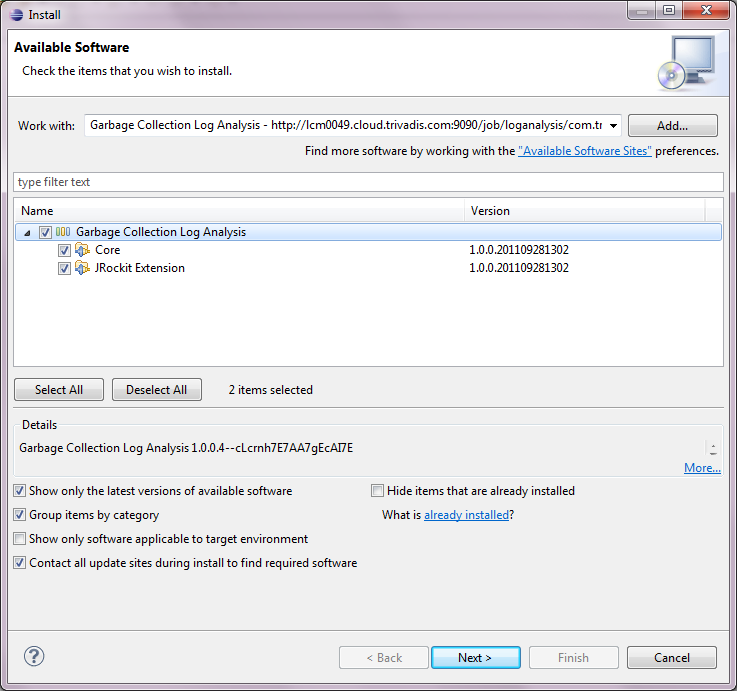
\includegraphics[width=10cm]{images/tutorial_install01}
        	\caption{Installation Garbage Collection Log Analyse}
\end{figure}

\section{Update (FRQ-02)}
Ein Update entspricht prinzipiell einer Neuinstallation der Software. Die einzelnen Module werden zur Laufzeit ausgewechselt und deren Classloaders ausgewechselt. Der Update-Bildschirm unterscheidet sich nur marginal vom Installations-Bildschirm, er ist aber über einen eigenen Menü-Eintrag aufrufbar.
 \begin{figure}[H]
  	\centering
    	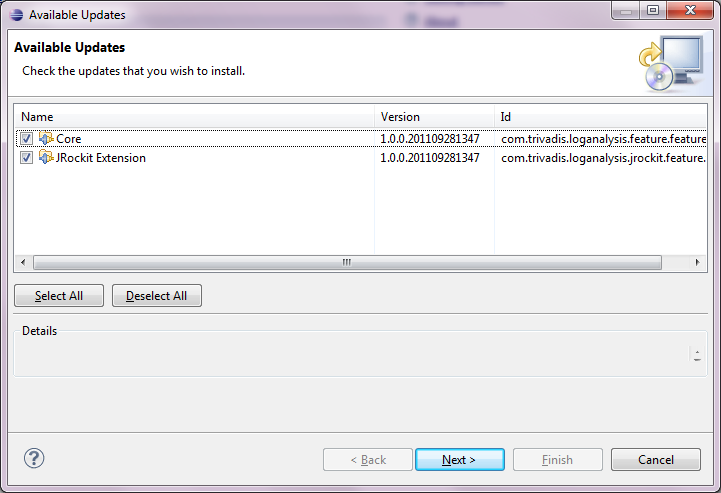
\includegraphics[width=10cm]{images/tutorial_update01}
        	\caption{Update Garbage Collection Log Analyse}
\end{figure}

\subsection{Datei importieren (FRQ-03)}
Die Dateien werden in eine eigene View importiert. Views sind programmierbare Komponenten (Ansichten) und können durch das Plugin deklarativ registriert werden. Sie stehen anschliessend dem Benutzer zur Verfügung. Das Speichern und Wiederherstellen des Zustands dieser View findet über das von Eclipse implementierte Memento-Pattern (siehe Anhang \ref{memento}) statt. Der Import findet über einen Wizard\footnote{Eclipse bietet die Möglichkeit, mit sehr geringem Aufwand Import- und Export-Wizards zu erstellen. Nur die GUI-Funktionalität muss implementiert werden.} statt. Der Benutzer wählt das Verzeichnis und die zu importierenden Logdateien aus. \begin{figure}[H]
  	\centering
    	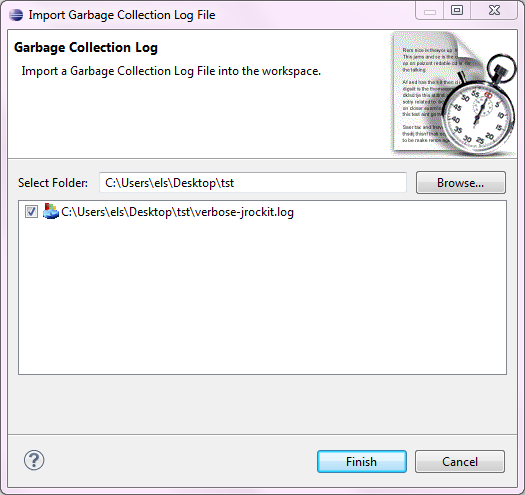
\includegraphics[width=10cm]{images/tutorial_importlog}
        	\caption{Logdatei importieren}
\end{figure}

\subsection{Datei einlesen (FRQ-05)}
Nachdem der Benutzer die Logdatei erfolgreich importiert hat, kann er sie mittels einem Doppelklick öffnen. Erst dann wird die Datei durch das Feature \textit{Core} eingelesen und im Arbeitsspeicher als Liste abgelegt. Die Speicherung als Liste ermöglicht es den Parsern, sequentiell oder durch die Angabe des Zeilenindexes auf die Daten zuzugreifen.

\subsection{Garbage Collection Logdatei parsen (FRQ-06)}
Die Log-Ausgaben des Memory-Moduls (Log-Level: info) werden mittels Regulären Ausdrücken geparst und in die strukturierte Form (siehe Abschnitt \ref{jrockit_domain_model}) gebracht. Die Analyse wird realisiert durch die Implementation eines Analyzers. Folgende Methoden müssen implementiert werden:
\begin{itemize}
\item \textit{boolean canHandleLogFile(IFileDescriptor)}
\item \textit{T process(IFileDescriptor descriptor, IProgress progress)}
\item \textit{String getEditorId()}.
\end{itemize}
Durch die Abstraktion des Interfaces \textit{Analyzer\textless T\textgreater} können später weitere Implementationen für neue Log-Formate erstellt werden.

\subsection{Standardauswertung anzeigen (FRQ-07)}
Für die importierten Dateien besteht die Möglichkeit, sie in der Standardauswertung anzuzeigen. Die Standardauswertung zeigt die im Konzept definierten Ansichten (siehe Abschnitt \ref{standardreport}):
\begin{itemize}
\item Übersicht Garbage Collection (FRQ-08)
\item Heap Kapazität (FRQ-09)
\item Dauer Garbage Collection (FRQ-10)
\end{itemize}


Als Beispiel die Ansicht des Heap-Diagrammes:
 \begin{figure}[H]
  	\centering
    	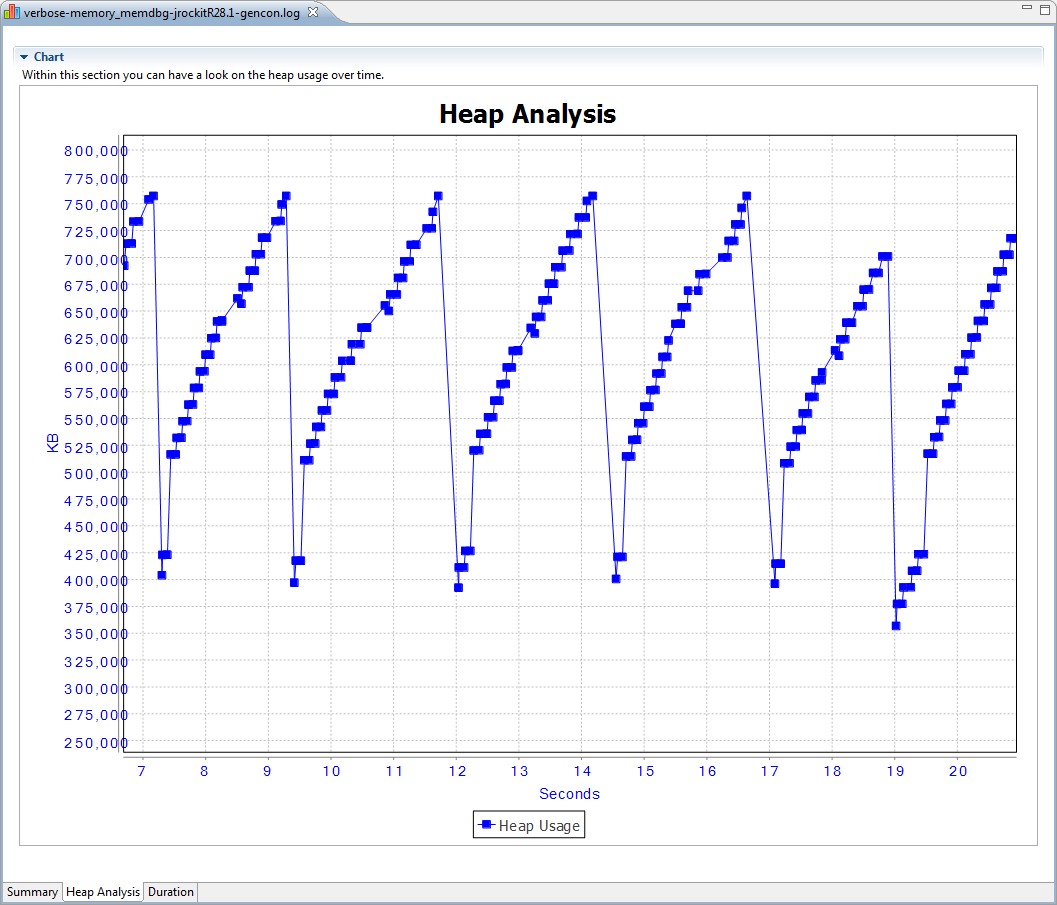
\includegraphics[width=15cm]{images/tutorial_standardreport_heapanalysis}
        	\caption{Standardauswertung: Heap Analyse}
\end{figure}

\subsection{Profil erstellen (FRQ-11)}
Profile können durch den Benutzer erstellt und an seine Bedürfnisse angepasst werden. Das Anpassen beinhaltet die Definition von eigenen Charts und deren Datenserien (FRQ-12). Speichern (FRQ-13), exportieren (FRQ-14) und importieren (FRQ-15) wird über das Memento-Pattern gemacht. Für weiter Informationen zum Memento siehe Anhang \ref{memento}.
 \begin{figure}[H]
  	\centering
    	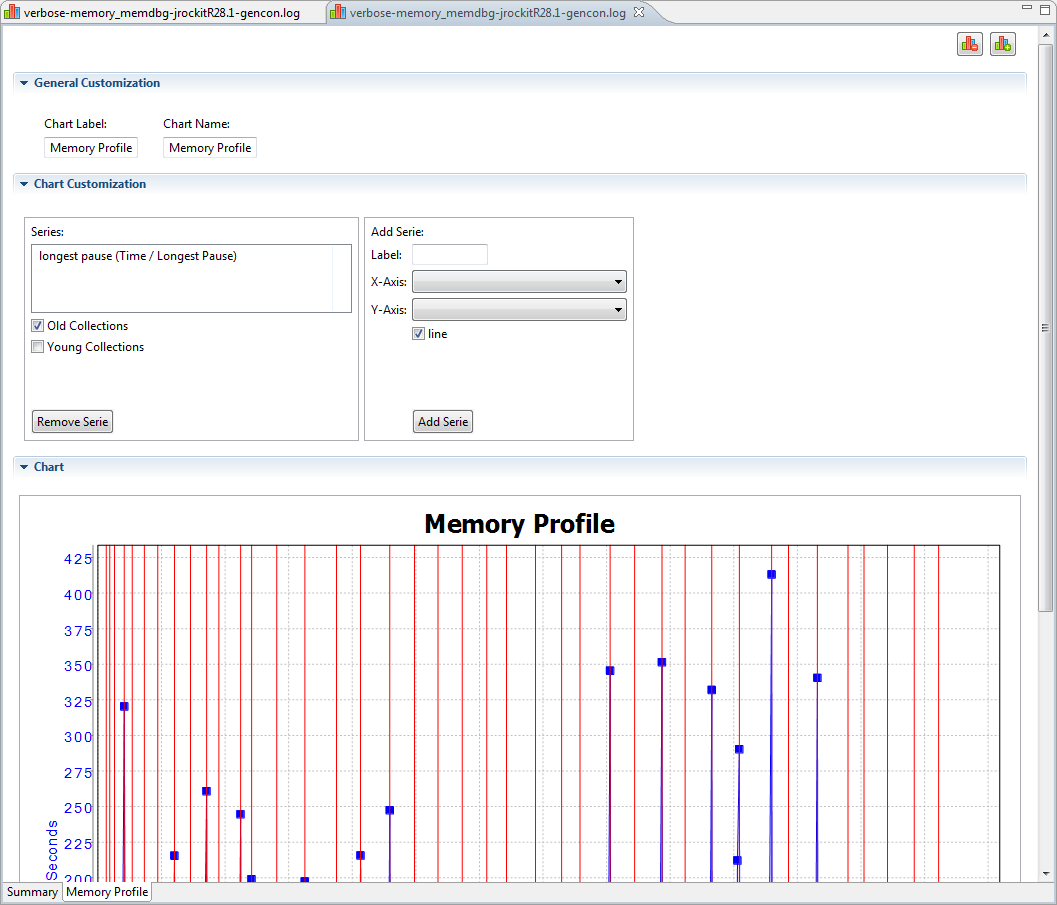
\includegraphics[width=15cm]{images/tutorial_custom_report}
        	\caption{Benutzerdefinierte Auswertung definieren}
\end{figure}

\subsection{Hilfesystem (FRQ-16)}
Das Hilfesystem wurde sowohl für die contextsensitive wie auch die indexbasierte Hilfe implementiert und kann stetig durch weitere Inhalte erweitert werden. Aktuell sind alle existierenden Hilfeseiten in den Sprachen Deutsch und Englisch umgesetzt, diese können aber sehr einfach um weitere Sprachen ergänzt werden. Die Sprache wird durch den Benutzer in der Datei \textit{eclipse.ini} definiert oder von der Java Laufzeitumgebung übernommen.

\section{Qualitätsanforderungen Software}
\subsection{Erweiterbarkeit (QRQ-S-01)}
Die Analyse für JRockit Logs wurde als Erweiterung implementiert. Es besteht die Möglichkeit, dass sich mehrere Erweiterungen bei der Basissoftware registrieren und damit auch das Parsen von anderen Logdateien möglich wird. Um ein neues Log-Format zu unterstützen, müssen folgende Schritte gemacht werden:
\begin{itemize}
\item Plugin erstellen in welches die Funktionalität getan wird.
\item Feature erstellen welches aus dem oben definierten Plugin besteht.
\item Feature auf der Update-Seite hinzufügen, so dass anschliessend auch dieses installiert werden kann.
\item Implementation des \textit{Analyzer}s und Konfiguration als Extension für den Extension-Point \textit{com.trivadis.loganalysis.analyzer}
\item erstellen des Auswertungsfensters, dafür können Super-Klassen der Basissoftware verwendet werden
\end{itemize}

\subsection{Testabdeckung (QRQ-S-02)}
Die Testabdeckung wurde zum jetzigen Zeitpunkt noch nicht ausgewertet, aber entspricht nicht den Anforderungen von 80 Prozent.
\subsection{Internationalisierung (QRQ-S-03)}
Viele der eingebauten Namen und Labels sind bereits zweisprachig (Englisch, Deutsch) definiert. Die restlichen müssen noch übersetzt und in die Sprachressourcen extrahiert werden.

\subsection{Usability (QRQ-S-04)}
Lange dauernde Operationen (einlesen, parsen der Daten) werden vom Eclipse-Framework asynchron gestartet. Dem Benutzer wird ein Progress-Monitor angezeigt. Es besteht also die Möglichkeit, den Prozess zu unterbrechen.

\subsection{Korrektheit (angezeigte Werte) (QRQ-S-05)}
Alle zu berechnenden Werte befinden sich im Datentyp \textit{BigDecimal}. Dies führt zwar zu einem erhöhten Ressourcenverbrauch, ist aber für die geforderte Genauigkeit nötig.